\chapter{Mesure du programme en fonctionnement}

\section{Introduction}
Cette section vise à venir meusrer différents élement lorsque la maquette est en mouvement. Ces mesures viennent directement analyser le comportement physique de la maquette.

\section{Mesure du temps de l'interruption principale}
L'une des premières hypothèses formulées a été que le code ne respectait pas le temps d'exécution alloué pour l'interruption complète. Il a donc été nécessaire de vérifier la validité des temps de cycle, de mesurer le temps consommé par chaque sous-routine, et de déterminer si l'interruption liée à la communication entre le DSP et l'ESP32 perturbait l'interruption principale.\\

Le protocole de mesure a consisté à évaluer le système avec les quatre inducteurs actifs, puis uniquement avec l'avant (inducteurs 1 et 2), et enfin uniquement avec l'arrière (inducteurs 3 et 4). Ces mesures ont été réalisées avec et sans l'activation de l'interruption de la liaison UART afin d'établir une comparaison. L'UART fut entièrement déscativé en mettant tout ce qui est en lien avec en commentaire. Pour rappel, la période de l'interruption principale est de 40~$\mu$s.

L'analyse temporelle se concentre sur quatre phases de l'interruption : premièrement, l'interruption dans son entièreté ; deuxièmement, le temps consommé par les conversions ADC ; troisièmement, le temps d'exécution de la machine d'états ; et enfin, le temps dédié à la mise à jour des signaux PWM. Les relevés ont été effectués à l'aide d'un oscilloscope en observant les commutations d'une broche de sortie (LED).\\

\subsection{Relevé des mesures}
Les mesures sont recensées dans le \autoref{tab:verif_temps_final} :

\begin{table}[H]
    \centering
    \resizebox{\textwidth}{!}{%
        \begin{tabular}{|l|c|c|c|c|c|c|}
            \hline
            \multicolumn{7}{|c|}{\textbf{Vérification des temps}}                                                                                                                                                                                                                                                                                                                                                                                                                                                  \\ \hline
            \multicolumn{1}{|c|}{\multirow{2}{*}{\textbf{Mesure}}} & \multicolumn{3}{c|}{\textbf{Avec UART}}                             & \multicolumn{3}{c|}{\textbf{Sans UART}}                                                                                                                                                                                                                                                                                                                                 \\ \cline{2-7}
            \multicolumn{1}{|c|}{}                                 & \begin{tabular}[c]{@{}c@{}}4 Inducteurs\\ {[}$\mu$s{]}\end{tabular} & \begin{tabular}[c]{@{}c@{}}Inducteurs\\ 1\&2 {[}$\mu$s{]}\end{tabular} & \begin{tabular}[c]{@{}c@{}}Inducteurs\\ 3\&4 {[}$\mu$s{]}\end{tabular} & \begin{tabular}[c]{@{}c@{}}4 Inducteurs\\ {[}$\mu$s{]}\end{tabular} & \begin{tabular}[c]{@{}c@{}}Inducteurs\\ 1\&2 {[}$\mu$s{]}\end{tabular} & \begin{tabular}[c]{@{}c@{}}Inducteurs\\ 3\&4 {[}$\mu$s{]}\end{tabular} \\ \hline
            Interruption globale                                   & 20                                                                  & 13.6                                                                   & 14.4                                                                   & 20.4                                                                & 14                                                                     & 14.4                                                                   \\ \hline
            ADC                                                    & 0.88                                                                & 0.86                                                                   & 0.84                                                                   & 0.88                                                                & 0.86                                                                   & 0.85                                                                   \\ \hline
            Machine d'état                                         & 13.2                                                                & 9.4                                                                    & 9.4                                                                    & 13.6                                                                & 9.6                                                                    & 9.6                                                                    \\ \hline
            PWM                                                    & 5.2                                                                 & 2.6                                                                    & 2.92                                                                   & 4.9                                                                 & 2.76                                                                   & 2.96                                                                   \\ \hline
        \end{tabular}%
    }
    \caption{Vérification des temps d'exécution avec et sans UART}
    \label{tab:verif_temps_final}
\end{table}

Les chronogrammes détaillés des mesures temporelles sont disponibles dans l'\autoref{an:MesTemps}.

\subsection{Analyse des résultats}
Comme l'illustre le \autoref{tab:verif_temps_final}, aucun temps d'exécution ne dépasse la période allouée à l'interruption. Une marge temporelle importante reste disponible. L'origine du dysfonctionnement global n'est donc pas liée à une surcharge du processeur, ce qui confirme la viabilité de l'interruption principale et de l'interruption de communication. Celles-ci n'entrent pas en conflit et s'exécutent sans se bloquer mutuellement.

Il aurait toute fois été plus interessant d'ajouter le trigger sur l'impulsion d'une durée minimum afin de voir si potentiellement l'interruption principale fut interrompue et aurais dès lors causer un problème.

\section{Mesure du comportement de la régulation de positions}
La régulation de position ne donnant pas un résutlat attendue, celle-ci fut dès lors "mesuré". La mesure est en réalité juste une récupération de différentes valeur sur une certaines durée. Cette mesure fut raéliser en employant l'ESP32 comme moyen d'enregistrer un CSV. Afin de transmettre les valeurs désiré, la fonction SendFloatAsText fut employé. Celle-ci fut agrandit pour permettre d'envoyer 10 valeurs. L'esp32 enregistra dès lors ces grandeurs sur une durée de 10s. Ce choix fut réaliser pour ne pas déborder sur la mémoire de l'ESP32. Plus tard, une communication UART fut plus tot réaliser entre la carte d'évaluation et un ordinateur pour ne pas avoir de problème de mémoire.

La mesure fut réaliser en activant uniquement l'avant ou l'arrière pour obtenir les résultats dans un etat stable de la maquette. La mesure fut réaliser, dans ces modes, par inducteur. Les mesures sont celle de la consigne de position, la position mesurée, l'erreur de positions, la consigne de force, l'intégrale de la consigne de positions et pour finir l'erreur.

\subsection{Mesure}
Les mesure résultante est présente dans les figures \ref{fig:RegPosInd1} à \ref{fig:RegPosInd4} :

\begin{figure}[H]
    \centering
    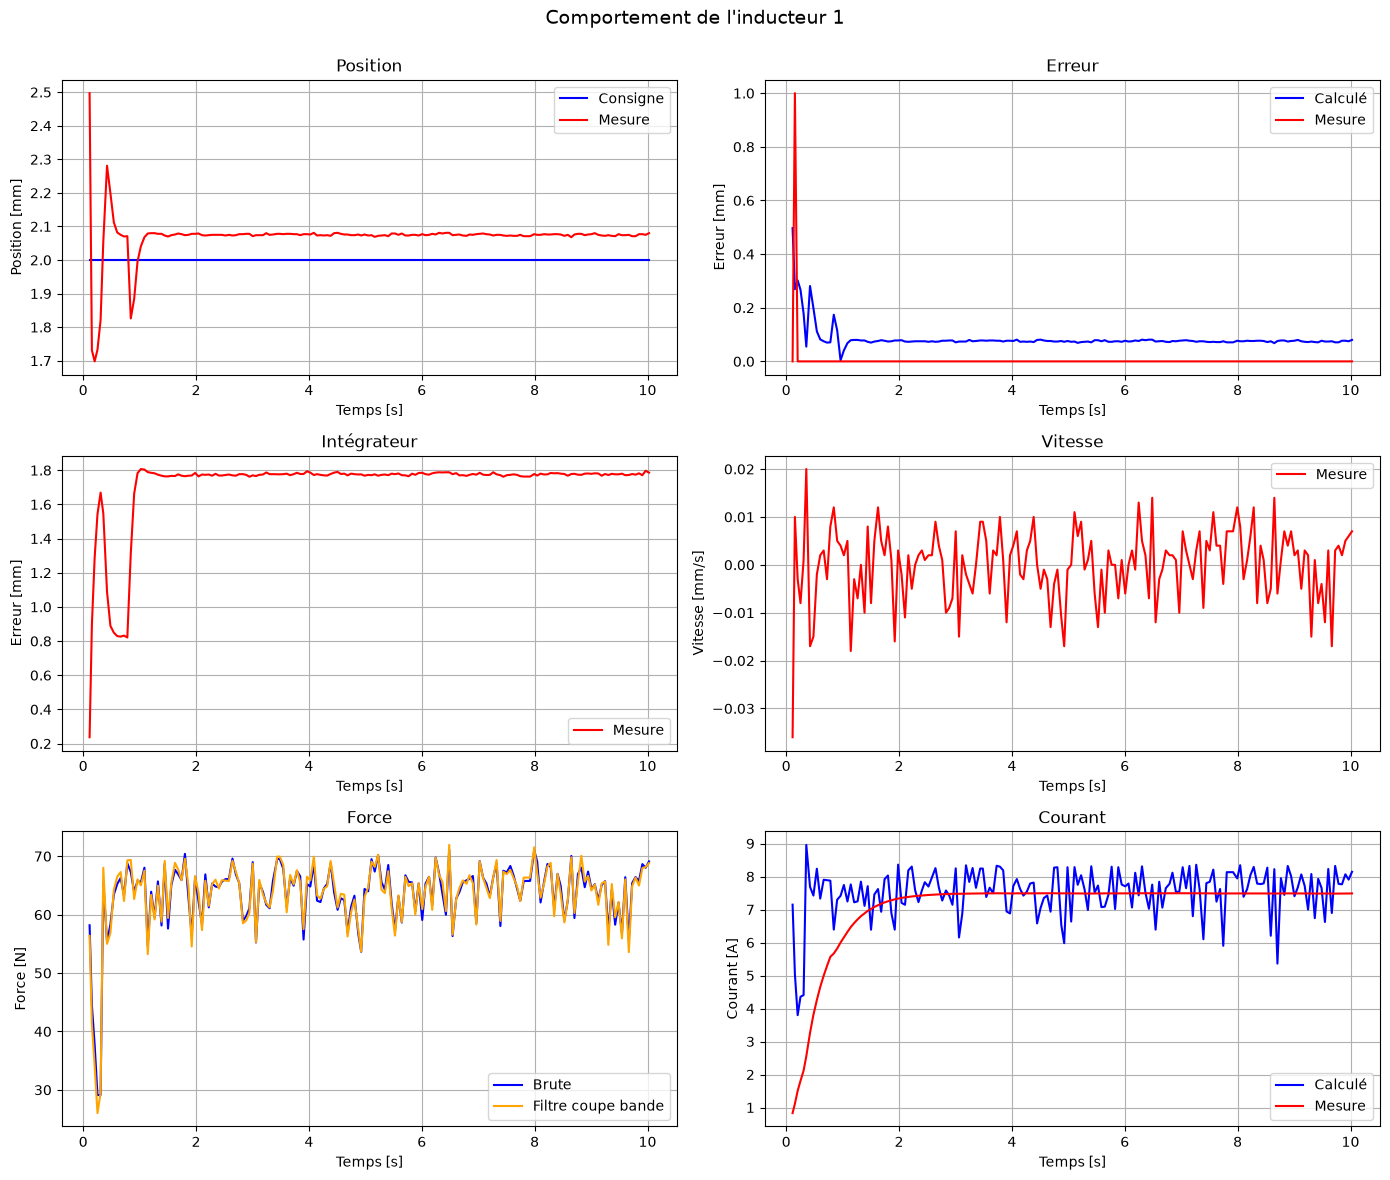
\includegraphics[width=1\linewidth]{assets/content/07-MesureProgPrinc/MesRegPos1.png}
    \caption{Évolution de la régulation de position pour l'inducteur 1}
    \label{fig:RegPosInd1}
\end{figure}

\begin{figure}[H]
    \centering
    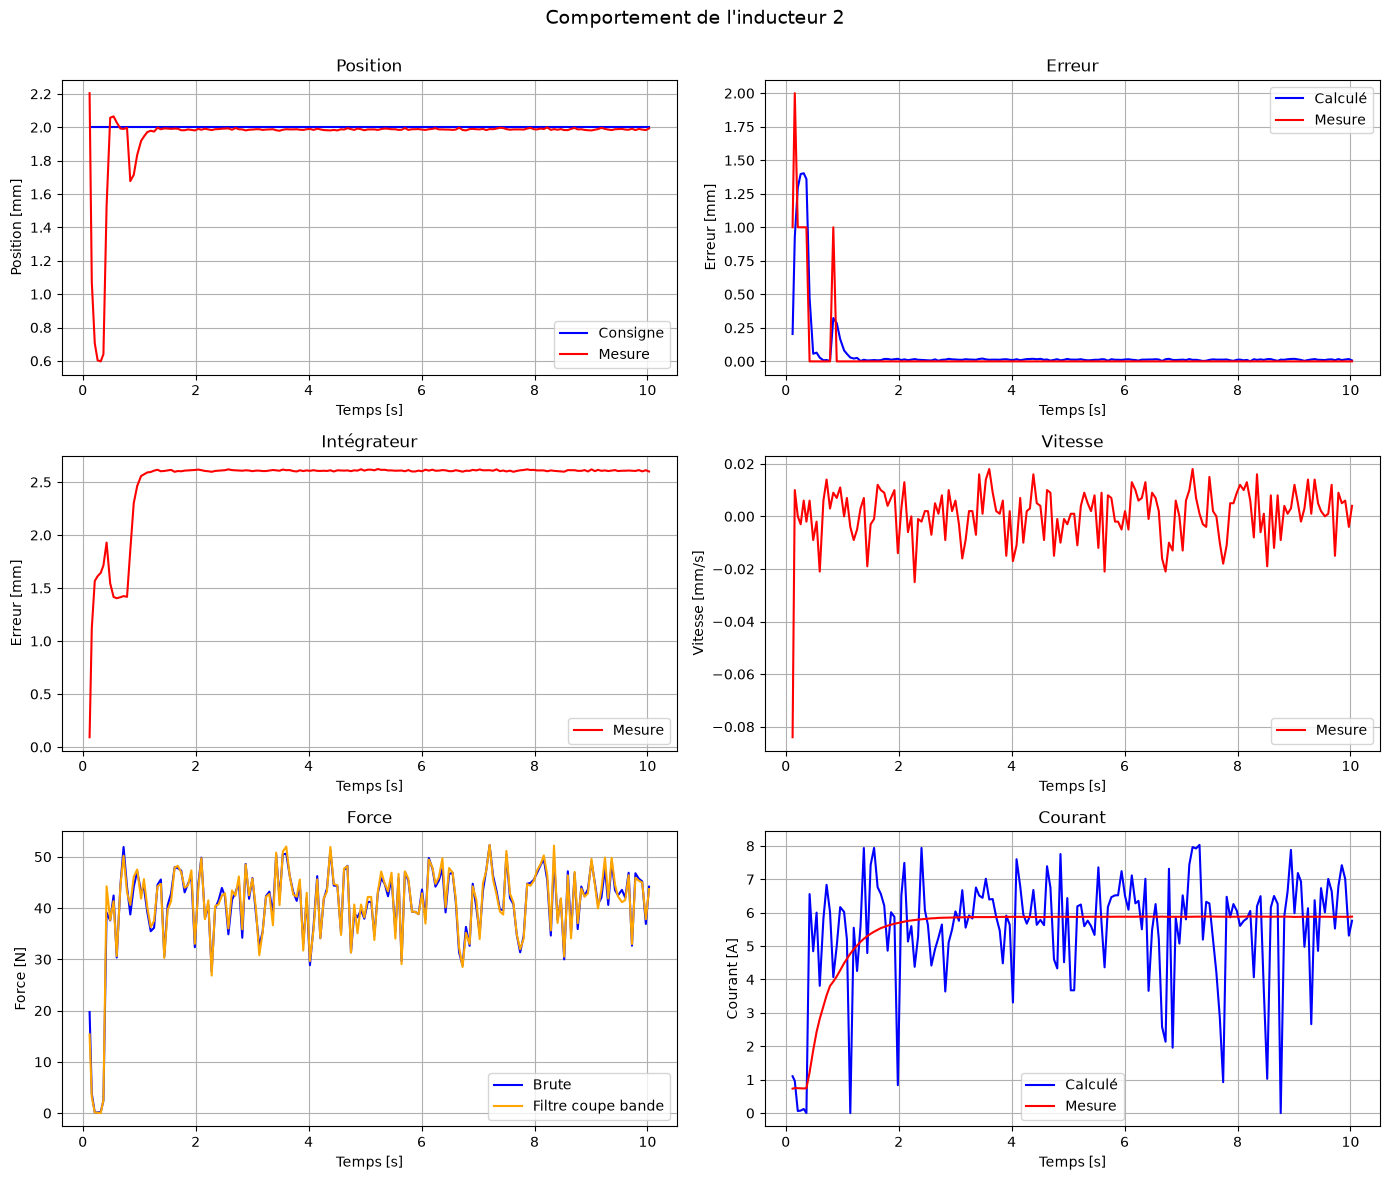
\includegraphics[width=1\linewidth]{assets/content/07-MesureProgPrinc/MesRegPos2.png}
    \caption{Évolution de la régulation de position pour l'inducteur 2}
    \label{fig:RegPosInd2}
\end{figure}

\begin{figure}[H]
    \centering
    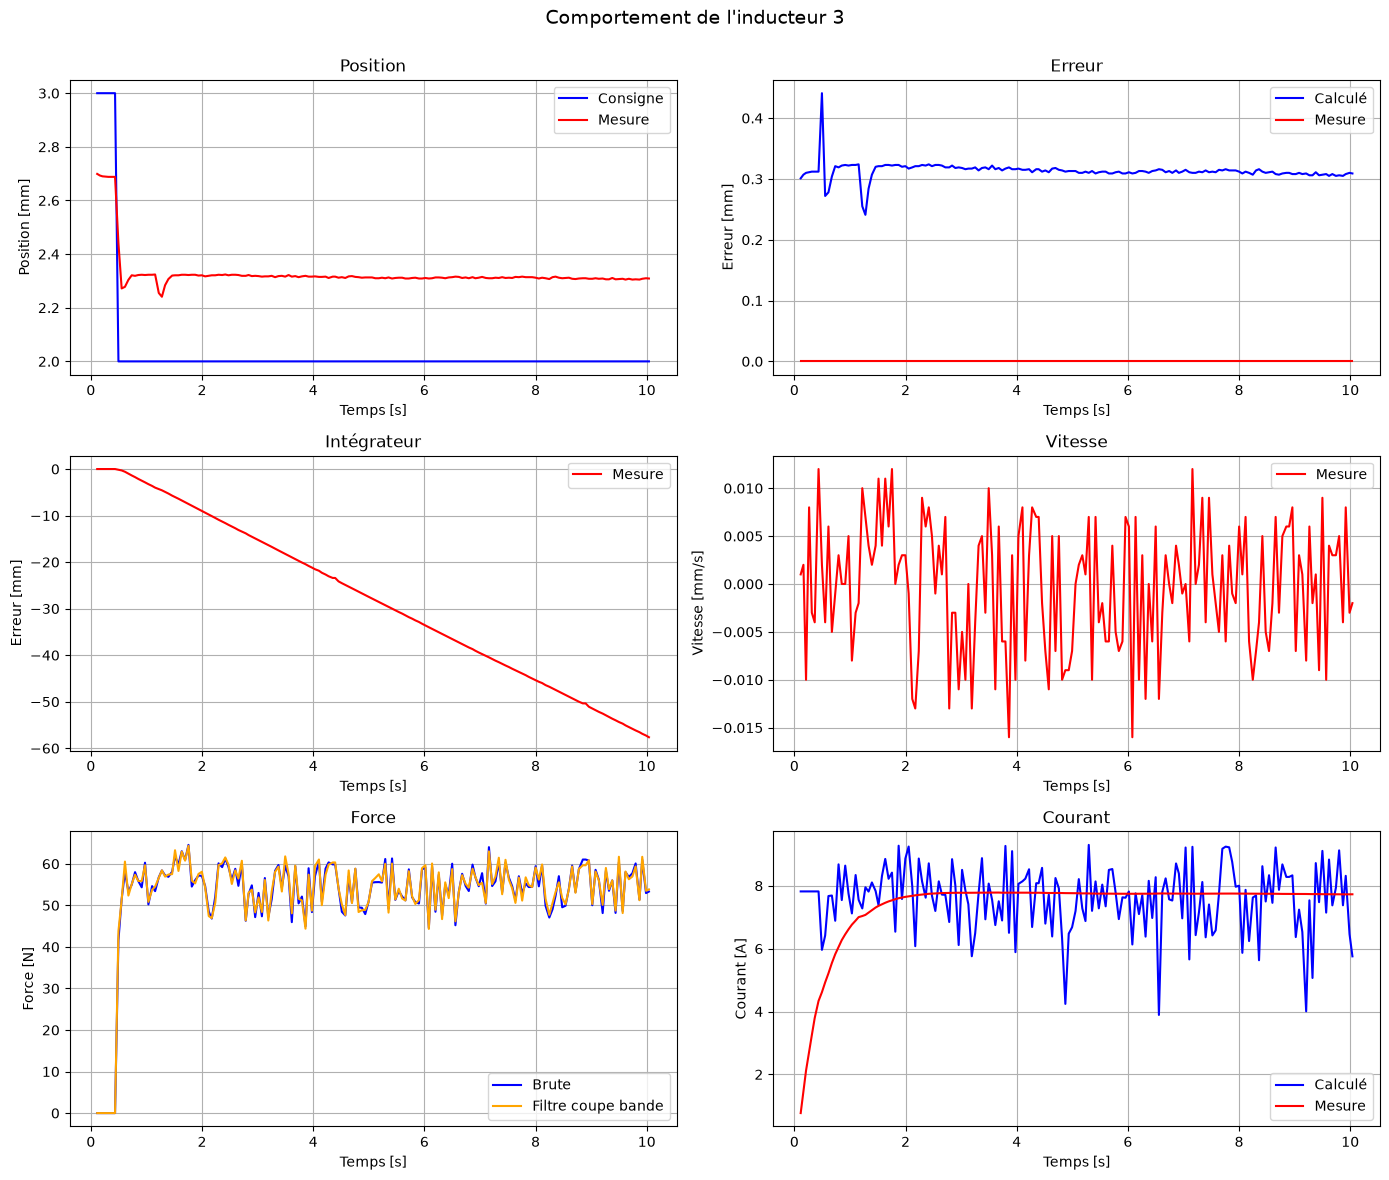
\includegraphics[width=1\linewidth]{assets/content/07-MesureProgPrinc/MesRegPos3.png}
    \caption{Évolution de la régulation de position pour l'inducteur 3}
    \label{fig:RegPosInd3}
\end{figure}

\begin{figure}[H]
    \centering
    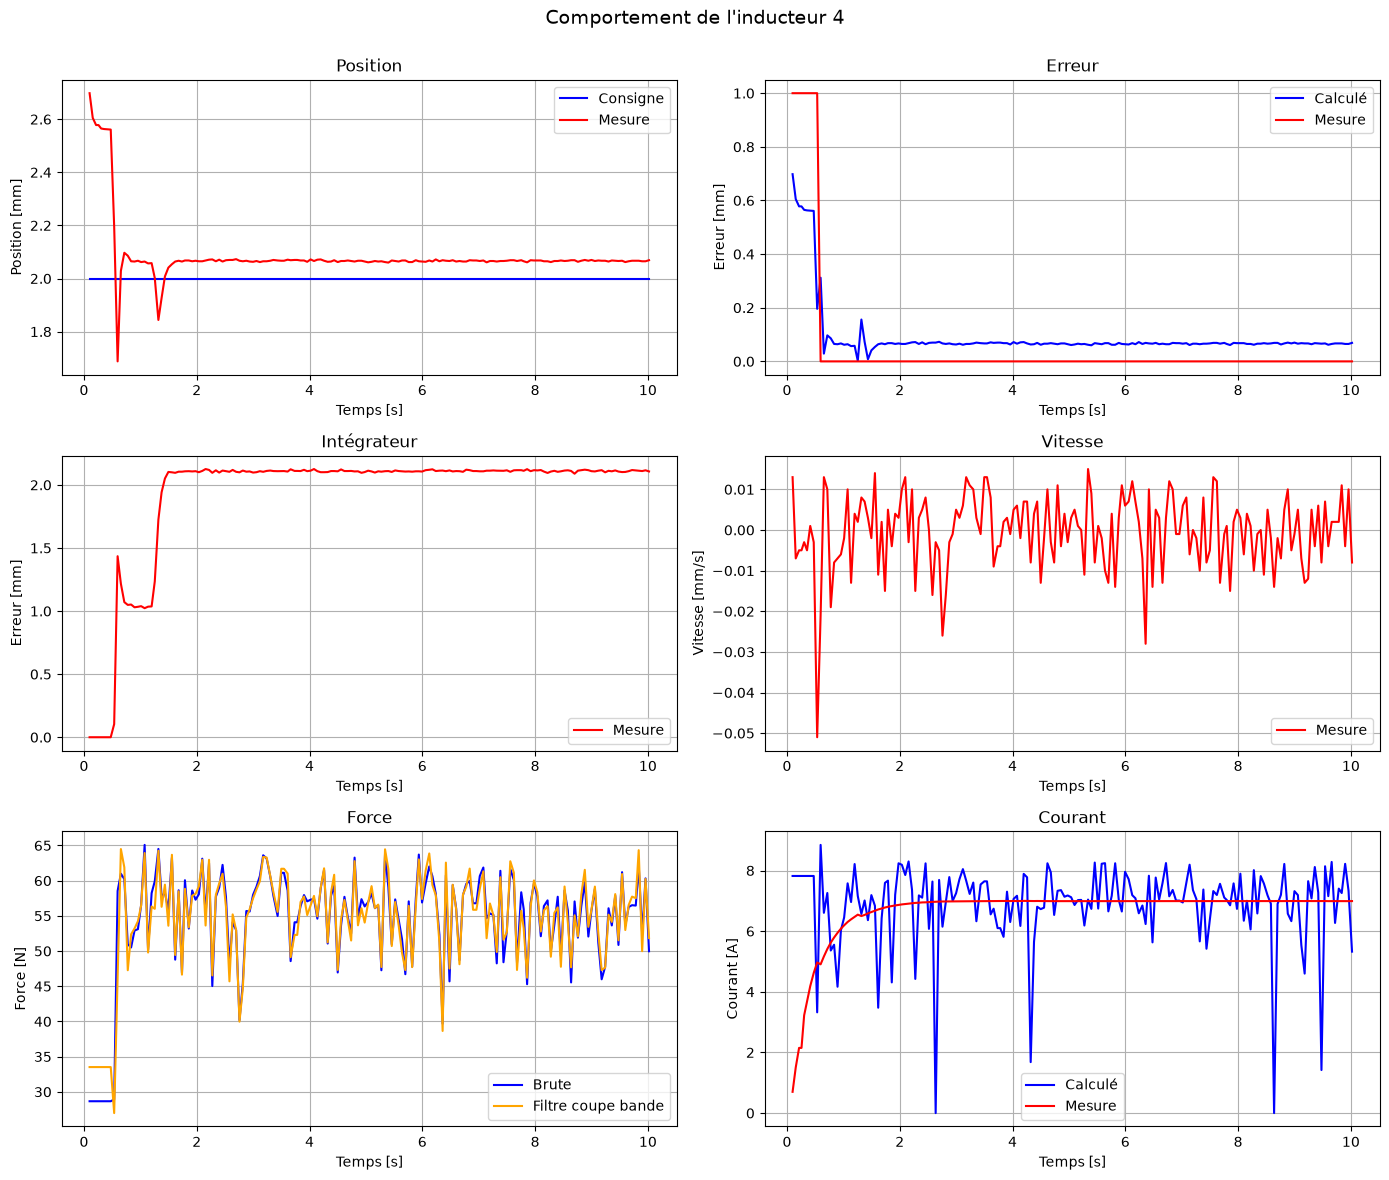
\includegraphics[width=1\linewidth]{assets/content/07-MesureProgPrinc/MesRegPos4.png}
    \caption{Évolution de la régulation de position pour l'inducteur 4}
    \label{fig:RegPosInd4}
\end{figure}

En venant se concentrer uniquement sur les consignes de force, il est possible de s'appercevoir que la consigne de force ne se situe pas vers la valeur théorique de la pensanteur. En effet, lorsque la maquette est en maintien, la force electromagnétique devrait être équivalent a la force de pesanteur. Ici celle-ci doit alors être equivalente à $F_{el} = 4.513\cdot9.81 = 44.3~N$. Hors cela est régulièrement dépassé ou meme inférieur a celle-la. Ceci est observable dans la \autoref{fig:ForceInd}:

\begin{figure}[H]
    \centering
    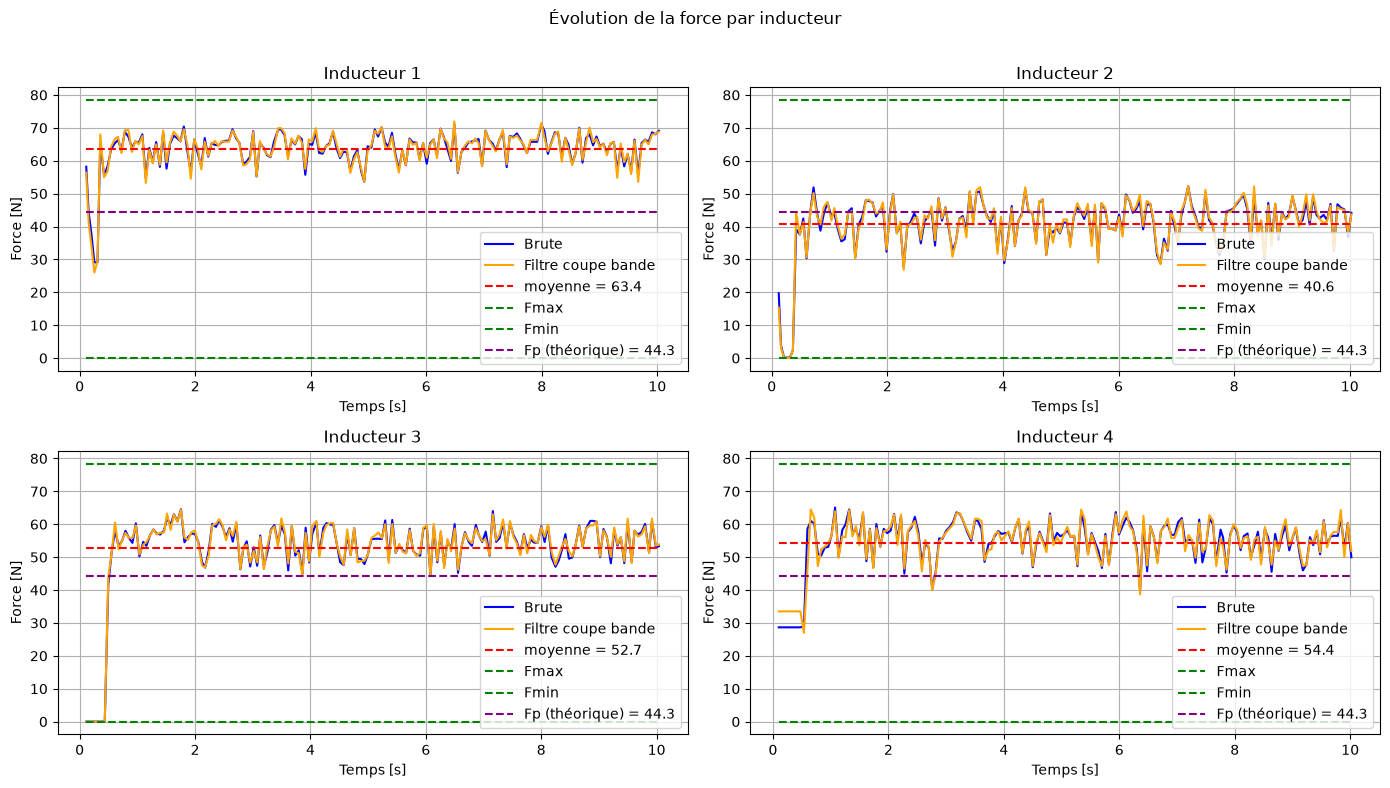
\includegraphics[width=1\linewidth]{assets/content/07-MesureProgPrinc/AnalyseForce.png}
    \caption{Évolution de la consigne de force par inducteur}
    \label{fig:ForceInd}
\end{figure}

Il est dès lors possible de réaliser un écart entre la valeur théorique et la moyenn. Ceci donne le \autoref{tab:forces_inducteurs} :

\begin{table}[H]
    \centering
    \begin{tabular}{l cccc}
        \toprule
        \textbf{Inducteur} & \textbf{Moyenne [N]} & \textbf{$F_p$ théorique [N]} & \textbf{Écart [N]} & \textbf{Écart [\%]} \\
        \midrule
        Inducteur 1        & 63.44                & 44.27                        & 19.17              & 43.29               \\
        Inducteur 2        & 40.63                & 44.27                        & -3.64              & -8.23               \\
        Inducteur 3        & 52.68                & 44.27                        & 8.41               & 18.99               \\
        Inducteur 4        & 54.43                & 44.27                        & 10.16              & 22.95               \\
        \bottomrule
    \end{tabular}
    \caption{Comparaison des forces moyennes et théoriques par inducteur}
    \label{tab:forces_inducteurs}
\end{table}

\subsection{Analyse des résultats}
Lors de l'observation


\begin{enumerate}
    \item Mesure courant et pos uniquement
    \item Mesure force, erreur etc
    \item Analyse resultat
\end{enumerate}
